\chapter{Identyfikacja z wykorzystaniem całek ruchu}\label{chap:identification}

\section*{Opis rozdziału}

W tym rozdziale będą przedstawione wyniki opublikowane w pracy~\cite{wieckowski.maska.2018}.
W cytowanej pracy, na przykładzie modelu Kitaeva, przedstawiono w jaki sposób można identyfikować \MZM\ dla układu opisanego dowolnym hamiltonianem, z perspektywy algorytmu bazującego na \acrshort{LIOM} opisanego w rozdziale~\ref{chap:LIOMs}.

\section{Układ  z oddziaływaniami wielociałowymi}

Znany jest fakt, że w niskowymiarowych układach oddziaływanie kulombowskie nie jest pomijalne i może efektywnie wpływać na właściwości takich układów~\cite{haldane.1981,gangadharaiah.braunecker.2011,manolescu.marinescu.2014,vuik.eeltink.2016,dominguez.cayao.2017}.
Takie oddziaływania są również istotne ze względów praktycznych.
Nieporządek jest obecny w~niemal wszystkich drutach półprzewodnikowych, a \MZM\ nie są całkowicie odporne na taki nieporządek~\cite{lutchyn.stanescu.2011,akhmerov.dahlhaus.2011,maska.gorczyca.2017}.
Średnie oddziaływania mogą stabilizować \MZM\ ze wzglądu na obecnośc takich zaburzeń w układzie~\cite{stoudenmire.alicea.2011,hassler.schuricht.2012,gergs.fritz.2016,dominguez.cayao.2017}.

Zasadniczo trudnym zadaniem jest identyfikacja \MZM\ w układach z oddziaływaniami wielociałowymi.
Często, pierwszą przesłanką jaką stawiają autorzy są badania degeneracji stanu podstawowego.
Należy tutaj przypomnieć, że degeneracja stanu podstawowego z podprzestrzeni z parzystą i nieparzystą liczbą cząstek ($\deltaE=0$) jest warunkiem \textit{koniecznym}, aby w układzie istniały \MZM.
Warunek \textit{wystarczający} jest nieco bardziej złożony.
Warunek ten bazuje na \glslink{LUE}{lokalnej unitarnej równoważności (ang. local unitary equivalance, LUE)} pomiędzy stanami układu z oddziaływaniami i stanami układu bez oddziaływań, w stanie topologicznym~\cite{chen.gu.2011}.
W celu pokazania równoważności \acrshort{LUE}, jeden ze stanów podstawowych musi się dać w sposób ciągły przetransformować do drugiego stanu, przy czym szczelina energetyczna powyżej stanu podstawowego powinna pozostać otwarta na całej ścieżce transformacji~\cite{fidkowski.kitaev.2010,katsura.schuricht.2015}.
Warunek równoważności \acrshort{LUE} sprawdza jedynie czy w danym układzie istnieją wspomniane w rozdziale~\ref{chap:LIOMs} \textit{soft} \MZM.
Soft \MZM\ są chronione tylko w temperaturach poniżej przerwy energetycznej --- warunek komutacji (definicja) \MZM\ z hamiltonianem $\hatH$ [równanie~\eqref{eq:MZMcom}] spełniony jest tylko i wyłącznie dla projekcji tego hamiltonianu na określoną niskoenergetyczną podprzestrzeń~\cite{alicea.fendley.2016}.

W Rozdziale~\ref{chap:LIOMs} przedstawiona została metoda, za pomocą której można identyfikować \textit{strong} \MZM\ w dowolnym układzie opisanym  hamiltonianem ciasnego wiązania.
W tym rozdziale przedstawiono działanie oraz skuteczność techniki opisanej w rozdziale~\ref{chap:LIOMs}.
Jako przykład, zbadany został model Kitaeva z oddziaływaniami wielociałowymi dla układu jednowymiarowego drutu z otwartymi warunkami brzegowymi (\acrshort{OBC}).
Taki model możemy interpretować jako fizyczną sytuację, w której nanodrut spoczywa na powierzchni nadprzewodnika typu \textit{p}.
Taki układ może być opisany za pomocą hamiltonianu~\eqref{eq:kitaev+V}.
W pracy ~\cite{wieckowski.maska.2018} badaliśmy następujący hamiltonian
\begin{equation}
    \hatH_{\text{Kitaev}+VW}^{\text{chain}} = 
    \sum_{i=1}^{\sites-1}\left[
    \left(\tuniform \, \aid \aii_{i+1} + \DeltaSCuniform\, \aid \aidii{i+1}\right)
    + \hc\right] -\muuniform \sum_{i=1}^{\sites}  \nz{i}
    +\Vuniform\sum_{i=1}^{\sites-1}   \nz{i} \nz{i+1}
    +\Wuniform\sum_{i=1}^{\sites-2}   \nz{i} \nz{i+2}
    ,\label{eq:kitaev+VW}
\end{equation}
gdzie $\Vuniform$, $\Wuniform$ to odpowiednio potencjały oddziaływań pomiędzy pierwszymi najbliższymi i drugimi najbliższymi sąsiadami.
We wszystkich wynikach prezentowanych w tym rozdziale przyjęto  $\HBAR=\tuniform=1$.

Poniżej podsumowano poszczególne kroki metody opisanej w rozdziale~\ref{chap:LIOMs} w celu identyfikacji \MZM\ w układzie:
\begin{enumerate}
    \item diagonalizacja hamiltonianu~\eqref{eq:kitaev+VW} \quad
    $U^\dagger\hatH_{\text{Kitaev}+VW}^{\text{chain}} U = \text{diag}(\Energy_n)$;
    \item konstrukcja macierzy $\corrGG_{ij}^{\timeTau} = (\bargammai^{\timeTau}|\gammaj)$ [równanie~\eqref{eq:corrGGdef}];
    \begin{enumerate}
        \item transformacja operatorów z bazy położeniowej Wanniera do bazy energetycznej hamiltonianu
        $\gammai \to U^\dagger \gammai U$;
        \item selekcja elementów [równanie~\eqref{eq:timeTauAvgDef}]
        $\bargammai^{\timeTau} = \sum_{|\Energy_n-\Energy_m|<\frac{1}{\timeTau}}(\gammai)_{nm} \qstate{n}\qstatet{m}$;
        \item wyznaczanie śladów [równanie~\eqref{eq:hilbertSchmidtInnerProductDef}]
        $(\bargammai^{\timeTau}|\gammaj) = \Tr(\bargammai^{\timeTau}\gammaj)/\Tr(\bbone)$;
    \end{enumerate}
    
    \item diagonalizacja macierzy $\corrGG_{ij}^{\timeTau}$ [równanie~\eqref{eq:KijEigen}]
    $\corrGG^{\timeTau} \alphaii_n = \lambdai_n(\timeTau) \alphaii_n$.
\end{enumerate}
Na końcu algorytm znajduje $D\sites$ modów Majorany $\Gammaii_n = \sum_i (\alphaii_{n})_i \gammai$, wraz ze stowarzyszoną wartością własną $\lambdai_n$, gdzie $n=1,\dots,D\sites$, $\sites$ to liczba węzłów w układzie, a $D$ to liczba stopni swobody związanych z węzłem sieci (w przypadku bezspinowych fermionów, w modelu Kitaeva $D=2$).
Jeśli $\lambdai_n=1$ to dana kombinacja operatorów Majorany jest zachowana w czasie, jest całką ruchu.
Dla $0 < \lambdai_n < 1$, część informacji związana z operatorem $\Gammaii_n$ jest zachowana dla dowolnie długich czasów.
W przypadku gdy $\lambdai_n=0$ infomacja związana z operatorem $\Gammaii_n$ jest całkowicie utracona.
Analiza takich wartości własnych $\lambdai_n$ powinna zostać poprzedzona odpowiednim skalowaniem rozmiarowym i czasowym.
Szczegóły takiego skalowania $\lambdai_n$ zostały opisane w sekcji~\ref{sec:sizeTimeScalling}, a wyniki przedstawione w sekcji~\ref{sec:finiteSizeScalingTheResults}.
W dalszej części pracy będziemy się zajmować najbardziej zachowanym operatorem, czyli o największej wartości
$\lambdai(\timeTau)=\max_n \lambdai_n(\timeTau)$.
Badane w pracy układy mogą posiadać do dwóch niezależnych \MZM, $\Gammaii_1$ oraz $\Gammaii_2$, które posiadają takie same wartości własne $\lambdai=\lambdai_1=\lambdai_2$

Na rysunkach~\ref{fig:lambdaResults1}(a), (b) oraz (d) przedstawiono zależność funkcji autokorelacyjnej $\lambdai(\timeTau)$ dla najbardziej stabilnej kombinacji $\Gammaii$. 
Badany układ, jednorodny łańcuch Kitaeva, może zwierać dwie \MZM\ znajdujące się na brzegach nanodrutu ~\cite{kitaev.2001,katsura.schuricht.2015,kells.2015}.
W tym rozdziale pokazano wyniki dla tylko jednej z nich, chyba że powiedziane zostanie inaczej.
Wyniki funkcji autokorelacyjnej dla drugiego najbardziej stabilnego operatora są identyczne.
Tak jak napisano w rozdziale~\ref{chap:LIOMs},
w przypadku braku oddziaływań wielociałowych, funkcje korelacyjne $\lambdai(\timeTau) = \thetaH{\timeTauM-\timeTau}$ [równanie~\eqref{eq:barGammaGammaMajcorr}].
Taka zależność $\lambdai(\timeTau)$  to wynik otrzymany czysto z~obliczeń numerycznych~\cite{wieckowski.maska.2018} i został przedstawiony na rysunku~\ref{fig:lambdaResults1}(a).
%Dla nieoddziałującego układu, z konsekwencji wycinania elementów macierzowych podczas uśredniania [równanie~\eqref{eq:timeTauAvgDef}], czas życia $\timeTauM$ jest proporcjonalny do odwrotności degeneracji stanu podstawowego $\timeTauM\,\propto\,\deltaE$.
Na rysunku~\ref{fig:lambdaResults1}(a) widać wspomniany charakter $\lambdai(\timeTau)$ --- wyniki dla układu bez oddziaływań.
W prezentowanym przykładzie przedstawiono zależność $\lambdai(\timeTau)$ dla kilku wybranych rozmiarów.
Należy tutaj zwrócić uwagę na skalę logarytmiczną $\timeTau$.
Widać, że $\timeTauM$ (odpowiada to wartości $\timeTau$ kiedy następuje zmiana wartości $\lambdai$ z $1$ na $0$) rośnie wykładniczo wraz z rozmiarem układu $\sites$ dla prezentowanego przykładu.
W konsekwencji dla prezentowanych wyników na rysunku~\ref{fig:lambdaResults1}(a) $\timeTauM\to\infty$ dla $\sites\to\infty$.
Oznacza to, że dla przedstawionych parametrów w układzie, w granicy termodynamicznej istnieją \MZM\ o nieskończonym czasie życia --- są to dokładne całki ruchu $[\hatH,\Gammaii]=0$.
Na rysunku~\ref{fig:lambdaResults1}(c) przedstawiono zależność $\timeTauM(\DeltaSCuniform)$ dla układu bez oddziaływań, dla skończonego układu $\sites=10$.
Szczególny przypadek, $\DeltaSCuniform=1$, odpowiada sytuacji, kiedy $\DeltaSCuniform=|\tuniform|$.
Dla takiego zestawu parametrów, tak jak pokazano w sekcji~\ref{sec:kitaev}, w modelu Kitaeva istnieją \MZM\ dokładnie komutujące z hamiltonanem nawet dla układów o skończonych rozmiarach, $\sites<\infty$.
Oczywiście, w konsekwencji prowadzi to do $\timeTauM\to\infty$ co tłumaczy widoczną asymptotę na rysunku~\ref{fig:lambdaResults1}(c).

Na rysunku~\ref{fig:lambdaResults1}(b), przedstawiono funkcję $\lambdai(\timeTau)$ analogicznie jak na rysunku~\ref{fig:lambdaResults1}(a), ale dla układu z oddziaływaniami wielociałowymi.
Funkcja $\lambdai(\timeTau)$ jest wygładzona w porównaniu do wyników bez oddziaływań, brakuje skokowego charakteru funkcji.
Pozycja wygładzonego skoku, również rośnie eksponencjalnie tak jak na rysunku~\ref{fig:lambdaResults1}(a), co sugeruje, że w granicy $\lim_{\timeTau\to\infty}\lim_{\sites\to\infty}\lambdai\approx1$.
Wydaje się, że w ogólności dla układów z oddziaływaniami wielociałowymi $\lambdai<1$, co sugeruje, że \MZM\ w układach z oddziaływaniami nie są dokładnymi całkami ruchu.
Interesujące, że oddziaływania mogą powodować zwiększenie skali czasowej kiedy $\lambdai$ jest \textit{duże} (np. $\lambdai\approx0.2$).
Na rysunku~\ref{fig:lambdaResults1}(d) przedstawiono wyniki $\lambdai$ dla różnych wartości potencjału $\Vuniform$.
Dla wybranych wartości $\Vuniform$ wspomniana skala czasowa zwiększa się o rząd wielkości.


\begin{figure}
    \centering
    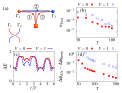
\includegraphics{04-Includes/Figures/LIOMS/fig1.pdf}
    \caption[%
Funkcja korelacyjna $\lambda(\tau)$ dla układu z oddziaływaniami oraz bez oddziaływań wielociałowych. 
Czas życia \textit{MZM}.
    ]{%
%
(a), (b), (d) Funkcja autokorelacyjna $\lambdai(\timeTau)$;
%
(a) $\Vuniform=0$, $\DeltaSCuniform=0.5$;
(b) $\Vuniform=0.2$, $\Wuniform=0.1$, $\DeltaSCuniform=0.5$;
(d) $\sites=12$, $\DeltaSCuniform=0.3$, $\Wuniform=\Vuniform/2$;
%
(c) czas życia \MZM $\timeTauM(\DeltaSCuniform)$ ($\sites=10$, $\Vuniform=\Wuniform=\muuniform=0$).
 %   
    }\label{fig:lambdaResults1}
\end{figure}

Przedstawiona metoda nie tylko bada korelację $\lambdai(\timeTau)$, ale równolegle znajduje kombinację najbardziej zachowanych operatorów $\Gammaii=\sum_i\alphai \gammai$.
W przypadku, gdy wszystkie elementy macierzowe hamiltonianu są rzeczywiste, spełniony jest następujący warunek ortogonalności\footnote{Dowód można znaleźć w~dodatku~\ref{chap:derivations}.}
\begin{equation}
    (\bargammai^+|\bargammaj^-)=0.\label{eq:gammaPlusGammaMinusOrthogonality}
\end{equation}
Wtedy w jednorodnym, układzie mogą  znaleźć się do dwóch \MZM, których bazy możemy podzielić na $\gammai^+$ oraz $\gammai^-$:
\begin{align}
\Gammaii^+ &= \sum_i \alphai^+\gammai^+,\\
\Gammaii^- &= \sum_i \alphai^-\gammai^-.
\end{align}
Macierz $\corrGG$ można wtedy zdekomponować na dwie mniejsze macierze $\corrGG=\corrGG^+\directsum\,\corrGG^-$, gdzie odpowiednio $\corrGG^\pm$ zawiera tylko korelacje zbudowane z operatorów $\gammai^\pm$.
Na rysunku~\ref{fig:lambdaResults2} przedstawiliśmy rozkłady przestrzenne \MZM, $\Gammaii^+$ oraz $\Gammaii^-$ w badanym układzie.
W celu weryfikacji poprawności stosowanej metody, porównano otrzymane wyniki z lokalną gęstością stanów (\acrshort{LDOS}) o zerowej energii~\cite{abrikosov.Dzyaloshinskii.1975,mahan.2000}
\begin{equation}
    \rho_i(\Energy=0) = -\tfrac1{\pi}\Im[\hat{\altmathcal G}_{ii}(\Energy=0)],
\end{equation}
gdzie funkcja Greena
\begin{equation}
   \hat{\altmathcal G}(\omega) = \frac{1}{\omega-\hatH_{\text{1-body}} + \iu \eta},
\end{equation}
gdzie $\hatH_{\text{1-body}}$ to hamiltonian jednocząstkowy --- zawierający wyrazy, które posiadają maksymalnie iloczyny dwóch operatorów kreacji lub anihilacji.
Na rysunku~\ref{fig:lambdaResults2}(a)--(b) przedstawiono porównanie znormalizowanego \acrshort{LDOS} z otrzymanymi współczynnikami $\alphai^\pm$ w przypadku bez oddziaływań wielociałowych.
Otrzymano perfekcyjną zgodność pomiędzy wynikami, co może świadczyć o skuteczności stosowanej metody.
Oczywiście metoda bazująca na \acrshort{LIOM} pozwala na badanie dowolnych układów, nawet tych z~oddziaływaniami wielociałowymi, co przedstawiono na rysunku~\ref{fig:lambdaResults2}(c)--(d).
Wyniki przedstawione na rysunkach~\ref{fig:lambdaResults2}(c)--(d) tłumaczą dlaczego na rysunku~\ref{fig:lambdaResults1}(d) widzimy zwiększenie  o~rząd wielkości skali dla którego $\lambdai$ jest duże.
Oddziaływania mogą zwiększać lokalizację \MZM\ na krawędziach układu, co może być powodem  powiększania obszaru topologicznego.
Na skutek lokalizacji zmniejsza się przekrywanie \MZM\ zwiększając ich czas życia.
Taki mechanizm przy dostatecznie dużym $\Vuniform$ przestaje funkcjonować i \MZM\ nie są obecne w układzie.

\begin{figure}
    \centering
    \includegraphics{04-Includes/Figures/LIOMS/fig2.pdf}
    \caption
    [Rozkład przestrzenny MZM]
    {Rozkład przestrzenny \MZM\ $\Gammaii^+,\,\Gammaii^-$.
    (a)--(b) Porównanie rozkładu przestrzennego $\alphai$ z normalizowanym \acrshort{LDOS}, układ bezoddziaływań $\Vuniform=\Wuniform=0$;
    (c)--(d) wyniki dla $\Wuniform=\Vuniform/2\neq0$.
    }
    \label{fig:lambdaResults2}
\end{figure}

\begin{figure}
    \centering
    \includegraphics{04-Includes/Figures/LIOMS/fig3.pdf}
    \caption
    [Porównanie degeneracji stanu podstawowego, szczeliny energetycznej z funkcją autokorelacją $\lambda(\tau)$ w funkcji $\mu$ i $V$.]
    {%
    Wyniki dla $\DeltaSCuniform=1$.
    (a) Degeneracja stanu podstawowego $\deltaE$ [równanie~\eqref{eq:degeneracyExtrapolation}];
    (b) szczelina energetyczna $\DeltaE$ [równanie~\eqref{eq:gapExtrapolation}];
    (c)--(d) funkcja autokorelacyjna $\lambdai$ dla różnych $\timeTau$ ($\sites=12$).
    }
       \label{fig:lambdaResults3}
\end{figure}


\begin{figure}
    \centering
    \includegraphics{04-Includes/Figures/LIOMS/fig4.pdf}
    \caption
    [Porównanie degeneracji stanu podstawowego, szczeliny energetycznej z funkcją autokorelacją $\lambda(\tau)$ w funkcji $\Delta$ i $V$.]
    {%
    Wyniki dla $\muuniform=0$.
    (a) Degeneracja stanu podstawowego $\deltaE$ [równanie~\eqref{eq:degeneracyExtrapolation}];
    (b) szczelina energetyczna $\DeltaE$ [równanie~\eqref{eq:gapExtrapolation}];
    (c)--(d) funkcja autokorelacyjna $\lambdai$ dla różnych $\timeTau$ ($\sites=12$).
    }
       \label{fig:lambdaResults4}
\end{figure}

\begin{figure}
    \centering
    \includegraphics{04-Includes/Figures/LIOMS/fig5.pdf}
    \caption
    [Skalowanie rozmiarowe funkcji autokorelacji $\lambda(\tau)$ w funkcji $\Delta$ i $V$.]
    {%
    Wyniki dla $\muuniform=0$, $\Wuniform=\Vuniform/2$.
    Funkcja autokorelacyjna $\lambdai$ dla różnych $\sites$
    (a) $8$;
    (b) $10$;
    (c) $12$;
    (d) $\infty$.
    Konturem w (d) zaznaczono $\lambdai=0.8$.
    }
       \label{fig:lambdaResults5}
\end{figure}

Dalej w celu  weryfikacji metody, porównano wyniki $\lambdai$ z warunkiem koniecznym --- degeneracji stanu podstawowego $\deltaE$ z sektorów z parzystą i nieparzystą liczbą cząstek --- oraz warunkiem wystarczającym --- \acrshort{LUE}.
W tym celu oszacowano degenerację stanu podstawowego $\deltaE$ oraz szczelinę energetyczną $\DeltaE$ w granicy termodynamicznej.
Poniżej przedstawiono schemat postępowania w celu wyznaczenia $\deltaE$ oraz $\DeltaE$.
Oszacowania dokonano poprzez skalowanie rozmmiarowe (\acrshort{FSS}) wyznaczając dla rozmiarów $\sites=8,10,\dots,20$, degenerację stanu podstawowego 
\begin{equation}
    \deltaE(\sites) = \Energy^e_0(\sites)-\Energy^o_0(\sites), \label{eq:degeneracyFinite}
\end{equation}
oraz dwie szczeliny energetyczne:
\begin{align}
    \DeltaE_e(\sites) &= \Energy_1^e(\sites)-\Energy_0^e(\sites),\label{eq:gapFinite1}\\
    \DeltaE_o(\sites) &=
    \Energy_1^o(\sites)-\Energy_0^o(\sites),\label{eq:gapFinite2}
\end{align}
gdzie $\Energy_0^{e,o}$ to energia stanu podstawowego z odpowiednio sektora z parzystą oraz nieparzystą liczbą cząstek.
Analogicznie $\Energy_1^{e,o}$  odpowiada energii pierwszego stanu wzbudzonego w odpowiednich sektorach.
Szczeliny energetyczne dla typowego układu powinny zanikać liniowo wraz z odwrotną liczbą węzłów $\sites$.
Do wyznaczenia $\DeltaE(\infty)$ dokonywaliśmy następującego dopasowywania funkcji $\DeltaE(\sites) = A \tfrac{1}{\sites}+\DeltaE(\infty)$.
Z drugiej strony degeneracja w obrębie obszaru topologicznego powinna zanikać wykładniczo.
Do wyznaczenia $\deltaE(\infty)$ wykorzystano funkcję wykładniczą
$\deltaE(\sites) = A\exp(-B\sites)+\deltaE(\infty)$.
Poza obszarem topologicznym, dopasowanie takich funkcji obarczone jest dużym błędem dopasowania $\sigma_{\deltaE}$, $\sigma_{\DeltaE}$.
Jako miarę degeneracji w granicy termodynamicznej przyjęto następującą wielkość
\begin{equation}
    \deltaE = |\deltaE(\infty)|+\sigma_{\deltaE} \label{eq:degeneracyExtrapolation}
\end{equation}
Jako dolne oszacowanie obszaru z degeneracją stanu podstawowego przyjęto  $\deltaE\ll 1$.
Równoważność \acrshort{LUE} zakłada, że  szczelina energetyczna nie zamyka się na całej ścieżce do obszaru topologicznego przy $\Vuniform=0$.
Jako dolne oszacowanie obszaru \acrshort{LUE} przyjęto
\begin{equation}
    \DeltaE = \min[\DeltaE_e(\infty),\DeltaE_o(\infty)]-\sigma_{\DeltaE}.
    \label{eq:gapExtrapolation}
\end{equation}
Wyniki $\deltaE$ oraz $\DeltaE$ dla układu $\DeltaSCuniform=1$ w funkcji $\muuniform$ oraz $\Vuniform$ zostały przedstawione na rysunkach~\ref{fig:lambdaResults3}(a)--(b).
Proces ekstrapolacji funkcji z pewnością obarczony jest błędami co można zauważyć na rysunku~\ref{fig:lambdaResults3}(a)  --- ukazują to niejednorodne czerwone obszary.

Na rysunkach~\ref{fig:lambdaResults3}(c)--(d) przedstawiono wyniki dla funkcji autokorelacyjnej $\lambdai$.
W odróżnieniu od wyników na rysunkach~\ref{fig:lambdaResults3}(a)--(b), które klasyfikują soft \MZM, wyniki na rysunkach~\ref{fig:lambdaResults3}(c)--(d) mogą posłużyć do znalezienia obszaru występowania strong \MZM. 
Otrzymane wyniki potwierdzają, że zarówno obszar występowania soft jak i strong \MZM\ poszerza się w zakresie $\muuniform$ na skutek oddziaływań wielociałowych~\cite{stoudenmire.alicea.2011}.





Na rysunku~\ref{fig:lambdaResults4} przedstawiono analogiczne wyniki jak na rysunku~\ref{fig:lambdaResults3}, ale dla $\muuniform=0$ i~różnych wartości $\DeltaSCuniform$.
Na rysunkach~\ref{fig:lambdaResults4}(c)--(d) dla $\DeltaSCuniform\ll1$, strong \MZM\ wydają się nieobecne nawet dla małych wartości oddziaływania $\Vuniform$.
To jest efekt skończonego rozmiaru, który wyjaśniono na rysunku~\ref{fig:lambdaResults5}.
Na rysunku~\ref{fig:lambdaResults5} wybrano $\timeTau=100$ i przedstawiono wyniki dla różnych $\sites$ wraz z ekstrapolowanym wynikiem dla $\sites\to\infty$.
Porównując wynik dotyczący warunku \acrshort{LUE} z  rysunku~\ref{fig:lambdaResults4}(b) z ekstrapolowanym wynikiem na rysunku~\ref{fig:lambdaResults5}(d),
obszar zwierający strong \MZM\ jest mniejszy od obszaru gdzie znajdują się soft \MZM.

\ornament

\begin{figure}
    \centering
    \includegraphics[width=0.7\textwidth]{04-Includes/Figures/LIOMS/S0.pdf}
    \caption
    [Kwadrat modułów elementów macierzowych mody Majorany.]
    {%
    Kwadrat modułów elementów macierzowych $|\Gammaii_{nm}|^2$ modów Majorany dla $\timeTau=100$, $\sites=12$, $\DeltaSCuniform=1$, $\Wuniform=\Vuniform/2$; 
    Poszczególne panele odpowiadają następującym $\Vuniform$ dla których otrzymano odpowiednie $\lambdai$:
    (a) $\Vuniform=0.5$, $\lambdai\simeq0.98$;
    (b) $\Vuniform=1.0$, $\lambdai\simeq0.92$;
    (c) $\Vuniform=2.0$, $\lambdai\simeq0.23$.
    }
    \label{fig:matrixElementsGamma}
\end{figure}

\section{Silność modów Majorany}

W tej sekcji przedyskutowano i jeszcze raz uargumentowano, że ten algorytm, rzeczywiście identyfikuje strong \MZM.
Z definicji strong \MZM: są to takie operatory $\Gammaii$, które komutują z hamiltonianem $\hatH$.
Z tego warunku wynika, że dla dowolnego stanu własnego, operator mapuje stan na stan o tej samej energii (co do efektów rozmiarowych) ale należącego do innego sektora parzystości~\cite{else.fendley.2017,goldstein.chamon.2012,kemp.yao.2017}, 
co można zapisać
\begin{equation}
    \Gammaii\qstate m = \eee^{\iu\phi_n}\qstate n,
\end{equation}
gdzie stany $\qstate n, \qstate m$ należą do sektorów o innej parzystości.
Tak jak napisano w rozdziale~\ref{chap:LIOMs}, wygodnie jest rozbić operator $\Gammaii$ na dwie części: 
część zachowaną $\barGammaii$ oraz na część ortogonalną $\barGammaii^{\perp}$ [równanie~\ref{eq:gammaConsPlusPerp}].
Komutacja części zachowanej z hamiltonianem wynika bezpośrednio z~konstrukcji takiego operatora
\begin{equation}
    [\hatH,\barGammaii] = \sum_{n,m:\Energy_n=\Energy_m}[\hatH,\Gammaii_{nm}\qstate n \qstatet m] = 
        \sum_{n,m:\Energy_n=\Energy_m}
        (\Energy_n-\Energy_m) \Gammaii_{nm}\qstate n \qstatet m = 0.
\end{equation}
Korzystając z relacji antykomutacji~\eqref{eq:majoranaCom0} oraz zakładając normę $\sum_i\alphai^2=1$ można pokazać, że
\begin{equation}
    \Gammaii^2 = \sum_{ij} \alphai \alphaj \gammai \gammaj = \tfrac12\sum_{ij}\alphai\alphaj\{\gammai,\gammaj\} = \sum_i \alphai^2 = 1.\label{eq:GammaSquare}
\end{equation}
W przypadku, gdy $\lambdai=1$, pokazano, że ta równość implikuje $\Gammaii=\barGammaii$.
W przypadku $\lambdai=1$  równanie~\eqref{eq:GammaSquare} spełnione jest dla $\barGammaii$: $\barGammaii^2 = 1$.
Korzystając z tego można pokazać, że dla dowolnego stanu $\qstate n$, spełnione jest równanie\footnote{Dowód można znaleźć w~dodatku~\ref{chap:derivations}.}
\begin{equation}
    1 = \qstatet n \barGammaii^2 \qstate n = \sum_{m:\Energy_n=\Energy_m} |\qstatet n \Gammaii \qstate m | ^2.\label{eq:parityMappingCondition}
\end{equation}
Z Równania~\eqref{eq:parityMappingCondition} wynika, że niezerowe elementy macierzowe $\qstatet n \Gammaii \qstate m$ są tylko dla stanów należących do sektorów o różnej parzystości.
Zakładając, że widmo energetyczne jest co najwyżej podwójnie zdegenerowane, dla każdego stanu $\qstate n$ o energii $\Energy_n$ z sektora o parzystej liczbie cząstek, istnieje stan $\qstate m$ o energii $\Energy_m$ z sektora o nieparzystej liczbie cząstek, taki, że $\Energy_n=\Energy_m$.
Korzystając z $\lambdai=1$, równania~\eqref{eq:parityMappingCondition}, oraz z założenia, że widmo energetyczne jest co najwyżej podwójnie zdegenerowane otrzymano wspomniany warunek na początku sekcji
\begin{equation}
        \Gammaii\qstate m = \eee^{\iu\phi_n}\qstate n,\label{eq:GammaStateMapping}
\end{equation}
co rzeczywiście potwierdza, że $\Gammaii$ jest strong \MZM.

Na rysunku~\ref{fig:matrixElementsGamma} przedstawiono elementy macierzowe $|\qstatet n \Gammaii\qstate m|^2=|\Gammaii_{nm}|^2$ w funkcji energii $\Energy_n,\,\Energy_m$.
Na panelu~\ref{fig:matrixElementsGamma}(a) przedstawiono wyniki dla układu zawierającego (prawie) strong \MZM\ --- $\lambdai\simeq0.98$.
Zgodnie z równaniem~\eqref{eq:GammaStateMapping}, dla każdego stanu własnego $\qstate n$ istnieje dokładnie jeden stan $\qstate m$ z innego sektora parzystości, taki że $|\Gammaii_{nm}|\simeq 1$ oraz $\Energy_n\simeq\Energy_m$.
Na środkowym panelu~\ref{fig:matrixElementsGamma}(b) przedstawiono wyniki dla układu z $\lambdai\simeq0.92$. 
W takim przypadku $\Gammaii$ nie jest strong \MZM.
Operator zawiera sporą część zachowaną $\barGammaii$ (patrz diagonalne elementy w bazie energetycznej) i nieco mniejszą część ortogonalną $\barGammaii^{\perp}$, reprezentowaną przez elementy pozadiagonalne.
Na ostatnim panelu~\ref{fig:matrixElementsGamma}(c) przedstawiono wyniki dla jeszcze mniejszej $\lambdai\simeq0.23$.
W części środkowej i maksymalnej spektrum energetycznego część zachowana jest zdecydowanie zmniejszona w porównaniu do poprzednich paneli ~\ref{fig:matrixElementsGamma}(a)--(b).
Największa część zachowana znajduje się w niskoenergetycznym spektrum co odpowiada niskim temperaturom.



\ornament

\section{Szczegóły skalowania rozmiarowego}\label{sec:finiteSizeScalingTheResults}

Zanim zostaną omówione szczegóły skalowania rozmiarowego (\acrshort{FSS}), skomentowano jeszcze warunek konieczny dla \MZM\ --- degenerację stanu podstawowego $\deltaE$.
Rysunek~\ref{fig:degeneracyExplanation}(a) wiernie odtwarza wyniki przedstawione w pracy~\cite{ng.2015}.
Na rysunkach~\ref{fig:degeneracyExplanation}(a)--(b) przedstawiono degenerację stanu podstawowego w sektorach z parzystą oraz nieparzystą liczbą cząstek odpowiednio dla układu z~$\Wuniform=0$ oraz $\Wuniform=\Vuniform/2$.
Na wykresach można zidentyfikować dwa obszary:
(\textit i) dwuwymiarowy obszar w okolicach punktu $\Vuniform=\muuniform=0$,
(\textit{ii}) linie wychodzące z obszaru (\textit i).
Na rysunku~\ref{fig:degeneracyExplanation}(a) struktura linii obszaru (\textit{ii}) jest słabo widoczna.
Dopiero przy niezerowym $\Wuniform$ na rysunku~\ref{fig:degeneracyExplanation}(b) struktura linii staje się bardziej widoczna.
Na rysunkach~\ref{fig:degeneracyExplanation}(c)--(d) przedstawiono wytłumaczenie pochodzenia tych linii --- zaprezentowano wyniki średniego obsadzenia stanu podstawowego $\langle\hatN\rangle$.
Wcześniej wspomniane linie z obszaru (\textit{ii}) nie są związane z \MZM\ i są również obecne w układzie $\DeltaSCuniform=0$, dla którego \MZM\ nie występują.
Linie te związane są z przekrywaniem się poziomów energetycznych z podprzestrzeni o~różnej liczbie cząstek parzystej oraz nieparzystej.
Te linie oddzielają obszary w których obsadzenia stanu podstawowego są blisko liczb naturalnych\footnote{Niewidoczne obsadzenia dla $0,1,\dots,\sites/2$ są dla ujemnych wartości $\muuniform$.} $0,1,2,\dots,\sites$.
Te wyniki podkreślają, jak istotne są warunki testowania \MZM.
Testowany warunek, degeneracja stanu podstawowego $\deltaE$, jest jedynie warunkiem koniecznym, ale niewystarczającym do określenia obecności \MZM\ w badanym układzie.

\begin{figure}
    \centering
    \includegraphics{04-Includes/Figures/LIOMS/S1.pdf}
    \caption
    [Średnia liczba obsadzeń $\langle \hat N \rangle$ oraz degeneracja stanu podstawowego $\delta E$]
    {
    (a)--(b) Degeneracja stanu podstawowego $\deltaE(\sites)$.
    (c)--(d) Średnia liczba obsadzeń $\langle \hatN \rangle$.
    Wyniki dla $\sites=8$, $\DeltaSCuniform=1$, (a), (c) $\Wuniform=0$, (b), (d) $\Wuniform=\Vuniform/2$.
    Czarne punkty na (c)--(d) dla parametrów dla których $|\deltaE(\sites)|<0.02$.
    }
    \label{fig:degeneracyExplanation}
\end{figure}


Podczas badania korelacji $\lambdai(\timeTau)$ istotnie ważna jest kolejność dokonywania skalowania rozmiarowego i czasowego.
Skalowanie rozmiarowe $\sites\to\infty$ powinno poprzedzać skalowanie czasowe $\timeTau\to\infty$.
Zgodnie z dyskusją przeprowadzoną w sekcji~\ref{sec:sizeTimeScalling}
w procesie relaksacji biorą udział dwa procesy:
proces związany z obecnością oddziaływań wielociałowych --- skala czasowa $\timeTauI$ --- oraz proces związany z oddziaływaniem modów Majorany --- skala czasowa $\timeTauM$.
Uwzględniając obydwa te procesy, funkcję autokorelacyjną $\lambdai(\timeTau)$ dopasowano korzystając z~następującej funkcji
\begin{equation}
    \lambdai_{\mathrm{fit}}(\timeTau) = 
    \frac{C}\pi\left
    \{
    \arctan\left[\left(\frac1{\timeTau}-\frac1{\timeTauM}\right)
    \timeTauI
    \right]
    +
    \arctan\left[\left(\frac1{\timeTau}+\frac1{\timeTauM}\right)
    \timeTauI
    \right]
    \right\}.
\end{equation}
Funkcja $\lambdai_{\mathrm{fit}}$ zawiera trzy parametry do dopasowania: $C$, $\timeTauI$ oraz $\timeTauM$.
Na rysunku~\ref{fig:fittingExamples} przedstawiono przykładowe dopasowania funkcji dla zestawu różnych parametrów.
Dopasowanie dobrze działa zarówno gdy: (a) dominuje jeden wybrany mechanizm relaksacji np. $\timeTauM\ll\timeTauI$ lub $\timeTauI\ll\timeTauM$,
(b) oba mechanizmy relaksacji mają przybliżone skale czasowe $\timeTauI\simeq\timeTauM$.


\begin{figure}
    \centering
    \includegraphics[width=0.7\textwidth]{04-Includes/Figures/LIOMS/S5.pdf}
    \caption
    [Wyniki funkcji autokorelacji $\lambda(\tau)$ wraz z dopasowaną funkcją $\lambda_{\text{fit}}$]
    {
    Porównanie funkcji autokorelacji $\lambdai(\timeTau)$ (punkty) wraz z dopasowaną funkcją $\lambdai_{\mathrm{fit}}$ (ciągłe linie).
    W tabeli zamieszczono dopasowane wartości $\timeTauM,\timeTauI$ odpowiednio dla $\Vuniform=0.0,\,0.3,\,0.7$. Wyniki dla $\DeltaSCuniform=0.3$, $\muuniform=0$, $\Wuniform=\Vuniform/2$, $\sites=12$.
    }
    \label{fig:fittingExamples}
\end{figure}

W celu badania układów w granicy termodynamicznej najpierw należy dokonać skalowania rozmiarowego (\acrshort{FSS}) współczynników relaksacji $1/\timeTauI$ oraz $1/\timeTauM$.
Na rysunkach~\ref{fig:scatteringRatesFSS}(a)--(d) przedstawiono skalowanie rozmiarowe takich współczynników dla wybranych przypadków.
Na panelach \ref{fig:scatteringRatesFSS}(a), (d) współczynniki $1/\timeTauM$ oraz $1/\timeTauI$ w granicy termodynamicznej dążą do zera.
Zatem wartość funkcji korelacyjnej $\lim_{\timeTau\to\infty}\lim_{\sites\to\infty}\lambda = C$.
Na panelach~\ref{fig:scatteringRatesFSS}(b), (c) odpowiednio współczynnik $1/\timeTauM$, $1/\timeTauI$ jest większy od zera w granicy termodynamicznej, co w konsekwencji prowadzi do $\lim_{\timeTau\to\infty}\lim_{\sites\to\infty}\lambda = 0$.
Jak napisano w sekcji~\ref{sec:kitaev}, \MZM\ w~modelu Kitaeva (w~przypadku bez oddziaływań) istnieją dla $|\muuniform|\le2\tuniform$, co udało się odtworzyć na rysunkach~\ref{fig:scatteringRatesFSS}(b), (d).

\begin{figure}
    \centering
    \includegraphics[width=0.7\textwidth]{04-Includes/Figures/LIOMS/S6.pdf}
    \caption
    [
    Skalowanie rozmiarowe współczynników relaksacji $1/\tau_{M}$ oraz $1/\tau_I$.
    ]
    {Skalowanie rozmiarowe współczynników relaksacji $1/\tau_{M}$ oraz $1/\tau_I$. Wyniki dla $\DeltaSCuniform=1$, $\Wuniform=0$.}
    \label{fig:scatteringRatesFSS}
\end{figure}

Po zakończonej procedurze \acrshort{FSS} można badać przybliżone wyniki dla funkcji korelacyjnej $\lambdai$ w granicy termodynamicznej, co zostało przedstawione na rysunku~\ref{fig:lambdaTermodynamicLimit}.
Wykresy~\ref{fig:lambdaTermodynamicLimit}(a)--(d) przedstawiają wyniki $\lambdai_{\mathrm{fit}}(\timeTau)$ dla których parametry $C$, $\timeTauM$, $\timeTauI$ zostały zastąpione ich aproksymowanymi wartościami w granicy termodynamicznej.
Procedura \acrshort{FSS} z pewnością obarczona jest sporymi błędami, o czym świadczyć może nieregularny kształt prezentowany na wykresach.
Na rysunku~\ref{fig:lambdaTermodynamicLimit}(d) przedstawiono przybliżone wartości $\lambdai$ dla $\timeTau\to\infty$.
Wydaje się, że informacja funkcji korelacyjnej $\lambdai$ jest przynajmniej częściowo zachowana dla dowolnie dużych czasów dla oddziaływań $\Vuniform<2$.




\begin{figure}
    \centering
    \includegraphics{04-Includes/Figures/LIOMS/S8.pdf}
    \caption
    [Ekstrapolowane funkcje autokorelacyjne $\lambda$ w granicy termodynamicznej.]
    {
    Ekstrapolowane funkcje autokorelacyjne $\lambdai(\timeTau)$ w granicy termodynamicznej $\lim_{\sites\to\infty}$. Wyniki dla $\DeltaSCuniform=1$, $\Wuniform=\Vuniform/2$.
    }
    \label{fig:lambdaTermodynamicLimit}
\end{figure}


\ornament

\section*{Podsumowanie}

W tym rozdziale został zaprezentowany przykład zastosowania algorytmu opisanego w~rozdziale~\ref{chap:LIOMs} do identyfikacji \MZM.
W tym celu zbadano model Kitaeva z oddziaływaniami wielociałowymi.
Porównano wyniki rozkładów przestrzennych \MZM\ otrzymane za pomocą tego algorytmu ze standardowymi wynikami \acrshort{LDOS}, jakie można otrzymać z wykorzystaniem formalizmu funkcji Greena.
Otrzymano perfekcyjną zgodność wyników pomiędzy dwiema metodami [rysunek~\ref{fig:lambdaResults2}(a)--(b)].
Dodatkowo nowa, zaproponowana w naszej pracy~\cite{wieckowski.maska.2018} metoda umożliwiła zbadanie wpływu oddziaływań wielociałowych na rozkłady przestrzenne \MZM.
Oddziaływania wielociałowe mogą zwiększać lokalizację \MZM\ na krawędziach układu [rysunek~\ref{fig:lambdaResults2}(c)--(d)].
Przedstawiona metoda pozwala na badanie silnych (lub prawie silnych) \MZM\ w układach z dowolnymi oddziaływaniami wielociałowymi.
Pokazano, że czasy życia takich modów, nawet w nieskończonych temperaturach, są wystarczająco długie i umożliwiają przechowywanie informacji.
Obszar występowania silnych \MZM\ zawiera się w obszarze występowania słabych \MZM, ale jest od niego mniejszy.
To oznacza, że nie wszystkie topologiczne stany są tak samo chronione i niekoniecznie tak samo dobrze nadają się do wykorzystania do przetwarzania kwantowej informacji.

\ornament


%%%%%%%%%%%%%%%%%%%%%%%
%% OTHER RESULTS, but not included
%\begin{figure}
%    \centering
%   \includegraphics{04-Includes/Figures/LIOMS/S2.pdf}
%    \caption{Caption}
%\end{figure}
%%%%%%%%%%%%%%%%%%%%%%%
%\begin{figure}
%    \centering
%    \includegraphics{04-Includes/Figures/LIOMS/S3.pdf}
%    \caption{Caption}
%\end{figure}
%%%%%%%%%%%%%%%%%%%%%%%
%\begin{figure}
%    \centering
%    \includegraphics{04-Includes/Figures/LIOMS/S4.pdf}
%    \caption{Caption}
%\end{figure}
%%%%%%%%%%%%%%%%%%%%%%%
%\begin{figure}
%    \centering
%    \includegraphics{04-Includes/Figures/LIOMS/S7.pdf}
%    \caption{Caption}
%\end{figure}
%%%%%%%%%%%%%%%%%%%%%%%
